% vim: fileencoding=utf-8:tw=0:noexpandtab:ts=4:sw=4
% -*- coding: utf-8 -*-

\documentclass[letterpaper, 10pt, conference]{ieeeconf}

\IEEEoverridecommandlockouts
\overrideIEEEmargins   

% packages
\usepackage[mathletters]{ucs}
\usepackage[utf8x]{inputenc}
\usepackage{graphicx}
\usepackage{microtype}
\usepackage{amsmath}
\usepackage{url}

% options
\graphicspath{{figures/}{generated-figures/}}

% commands
\newcommand{\fig}[1]{Figure~\ref{fig:#1}}
\newcommand{\Fig}[1]{Figure~\ref{fig:#1}}
\newcommand{\tbl}[1]{{Table}~\ref{fig:#1}}
\newcommand{\Tbl}[1]{{Table}~\ref{fig:#1}}
\newcommand{\sect}[1]{Section~\ref{sec:#1}}
\newcommand{\Sect}[1]{Section~\ref{sec:#1}}
\newcommand{\hypo}[1]{Hypothesis~\ref{hyp:#1}}
\newcommand{\Hypo}[1]{Hypothesis~\ref{hyp:#1}}
\newcommand{\algo}[1]{Algorithm~\ref{algo:#1}}
\newcommand{\Algo}[1]{Algorithm~\ref{algo:#1}}
\newcommand{\eq}[1]{Equation~\ref{eq:#1}}
\newcommand{\Eq}[1]{Equation~\ref{eq:#1}}

% title and authors

\title{\LARGE \bf
Localization of inexpensive robots with low-bandwidth sensors
}

\author{Shiling Wang$^{1}$ and Francis Colas$^{2}$ and Ming Liu$^{3}$ and Francesco Mondada$^{4}$ and Stéphane Magnenat$^{5}$% <-this % stops a space
\thanks{$^{1}$Shiling Wang is with ETH Zürich
        {\tt\small shilingwang0621@gmail.com}}%
\thanks{$^{2}$Fraucis Colas is with INRIA Nancy Grand Est
        {\tt\small francis.colas@inria.fr}}%
\thanks{$^{3}$Ming Liu is with City University of Hong Kong
        {\tt\small mingliu@cityu.edu.hk}}%
\thanks{$^{4}$Francesco Mondada is with Mobots, LSRO, EPFL
        {\tt\small francesco.mondada@epfl.ch}}%
\thanks{$^{5}$Stéphane Magnenat is with Mobots, LSRO, EPFL
        {\tt\small stephane@magnenat.net}}%
}

\begin{document}

\maketitle
\thispagestyle{empty}
\pagestyle{empty}

\begin{abstract}
Lorem ipsum...
\end{abstract}

\section{Introduction}

Driven by consumer products, electronics, motor and battery technologies have made tremendous progress in the last decades.
They are now available widely at a price making affordable mobile robots a reality.
This opens many new opportunities, in particular in the educational context.
Robots have been shown to be effective in supporting the teaching of knowledge such as mathematics, physics, computer science and engineering; and of skills such as problem solving and the scientific method~\cite{benitti2012explorin}.

Programmable platforms such as the LEGO Mindstorms, in the 300-400\,\$ price range, have been successfully used in classrooms worldwide, especially to teach engineering.
Yet, despite its high price tag, this platform has little perception capabilities; its longest-range sensor being a single ultrasound unit.
Cheaper products such as the Thymio~II (120\,\$) and Dash \& Dot (160\,\$) even lack such a long-range perception capability, and only provide local infrared sensors.
These are limited to sensing distances up to 15\,cm and measuring the grayscale intensity of a close object or the ground.
These products also lack a camera, because processing image would require extended memory and processing resources, which would increase their price significantly.
Therefore, all affordable educational robots (in the 100\,\$ range) lack long-range sensing capabilities.
In addition, dead-reckoning on these platforms is bad to non-existant, as proper wheel encoders are too expensive.
When dead-reckoning is provided, such as on the Thymio~II, it builds on approximate methods such as measuring the back electromotive force.
% A notable exception is the BeeBot, which uses proper dead-reckoning as its only sensor.
% But this robot can only follow pre-programmed trajectories, it is not able to react to external events.

The combined lack of long-range sensors and quality dead-reckoning prevents these robots from using state of the art localization algorithms, such as simulataneous localization and mapping.
This limits their educational use, in particular for the study of geometry, physics, and engineering; but also the building of advanced behaviours, such as several robots playing a staged story in a shared space.

This paper solves this problem.
We provide an obsolute positioning system using only approximate dead-reckoning and inexpensive infrared sensors measuring ground lightness.
Our solution builds on a recursive Bayesian filter, of which we propose both a dense and a sampling-based implementation.
We evaluate these using the Thymio~II mobile robot on a known black and white pseudo-random pattern, with ground truth provided by a Vicon tracking system.
In addition, we provide a theoretical contribution predicting the traveled distance necessary to localize the robot.
Finally, we show how users can draw their own ground images and use these to localise the robot.

\section{Related work}

Markov and Monte Carlo Localization, why not SLAM?

Localization techniques for cheap mobile robots.
The challenge of solving lovalization problem of cheap mobile robots is the sensor information is very limited.
Some approaches, such as \cite{prorok2012low, dias2013absolute}, solve localization problem of multiple cheap robots instead of a single robot by using collaborative sensors information.

In \cite{pinto2012localization}, Extended Kalman Filter algorithm is conducted in a LEGO NXT for the purpose of teaching undergraduate university students localization of mobile robots.
The localization environment is with several white walls and EKF uses information from infra-red sensors equipped on the robot.


\section{Material}
% Merge all three parts together. Datasets gather from two sources: gt and thymio. mention a bit of the frequency and speed. Trajectories detail: what kind of motion, also kidnapping. Total length should not over one column plus the figure. Figure need some explanation.

We run empirical experiments with the Thymio~II mobile robot localizing on a printed map.

Thymio~II is an open-source differential-wheeled mobile robot.
Its footprint is approximately $10 \times 10$ cm and it costs about 120\,\$.
About 10k units have been sold to date and are used in the context of computational thinking and engineering education~\cite{magnenat2012arso}.
It features many sensors; in the context of this project, only two ground infrared sensors are used. % TODO: ref figure
Thymio~II is programmed through the Aseba framework~\cite{aseba2011tmech}.
For this work, Aseba is connected to the \textsc{ros} framework\footnote{ROS (Robot Operating System): \url{http://www.ros.org/}}.

The map consists of a 150$\times$150\,cm pattern containing 50\,$\times$\,50 black and white random cells of 3$\times$3\,cm.
The pattern is generated randomly with an equal probability of black and white cells and without regularization.

To evaluation the performance of our localization algorithms, we record the ground-truth pose of the robot using a Vicon\footnote{\url{http://www.vicon.com/}} tracking system.
%to provide the ground-truth robot pose, consisting of $x$, $y$ coordinates and the heading $\theta$.
We use \textsc{ros} to synchronously record these along with sensor values and odometry information from Thymio.
During the dataset gathering, the robot move on the map with a speed of 3--5\,cm/s.
The data are gathered with an high enough frequency of 100\,Hz (ground-truth) and 10\,Hz (robot) for subsequent subsampling.
To fully explore the performance of the algorithm, we remote control the robot along several trajectories covering all possible motions.
An example trajectory is shown in \fig{dataset}.

\begin{figure}
\begin{center}
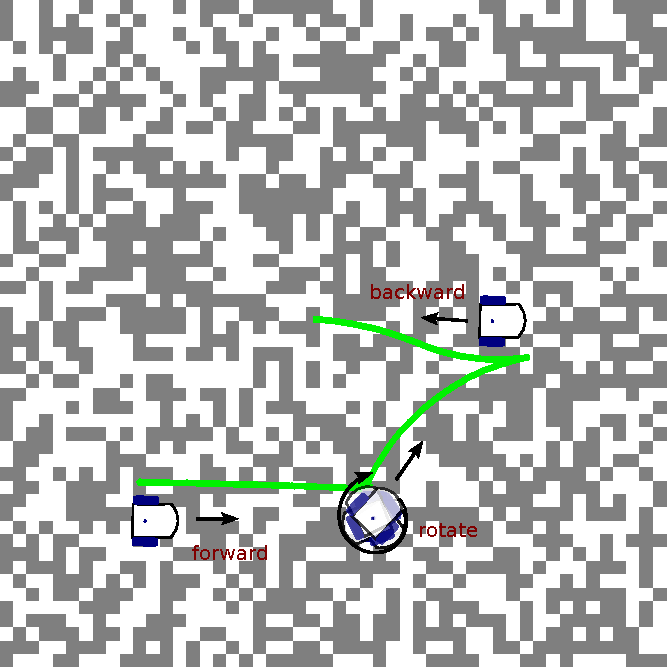
\includegraphics[width=0.4\textwidth]{dataset}
\caption{An example trajectory of the robot. The robot moves on the map with random black and white pattern with three different motions: going forward, going backward and rotating on spot.}
\label{fig:dataset}
\end{center}
\end{figure}

The motions of the robot can be classified into two different types, namely moving forward or backward (possible in arcs) and rotating on spot.
To test the algorithm's ability of recovering from catastrophic localization failures, we also conduct experiments with robot kidnapping by lifting the robot and moving it to another part of the map.

\section{Model}

\subsection{Variables}

The model uses the following variables:
\begin{itemize}
\item $X_{1:t}$ 2-D pose at times $1..t$.
The pose vector consists of $x,y$ coordinates and an angle $\theta$.
\item $Z_{1:t}$ observations at times $1..t$.
The observation consists of two sensors located at the bottom of the robot, measuring the intensity of the ground.
\item $U_{1:t}$ odometry at times $1..t$.
The odometry consists of the left and right wheel speeds.
\end{itemize}

\subsection{Joint probability}

We formulate the model as a recursive Bayesian filter.
Its joint probability is:
\begin{equation}
\begin{split}
& p(X_{1:t}, Z_{1:t}, U_{1:t}) = \\
& p(Z_t|X_t) p(X_t|X_{t-1}, U_{t}) p(U_t) p(X_{1:t-1}, Z_{1:t-1}, U_{1:t-1})
\end{split}
\end{equation}

\subsection{Question}

We want to estimate the pose $X_t$ at time $t$ knowing the observations $Z_{1:t}$ and the commands $U_{1:t}$:
\begin{equation}
\begin{split}
& p(X_t|Z_{1:t},U_{1:t}) = \frac{p(X_t,Z_t | Z_{1:t-1}, U_{1:t})}{p(Z_t|Z_{1:t-1}, U_{1:t})} \\
 &\propto p(Z_t | X_t) p(X_t | Z_{1:t-1}, U_{1:t}) \\
 &\propto p(Z_t | X_t) \sum_{X_{t-1}} p(X_t, X_{t-1} | Z_{1:t-1}, U_{1:t} ) \\
 &\propto p(Z_t | X_t) \sum_{X_{t-1}} p(X_t|X_{t-1}, U_t) p(X_{t-1} | Z_{1:t-1}, U_{1:t-1})
\end{split}
\end{equation}
%This is a recursive filter to estimate $X_t$ using the previous estimation $X_{t-1}$, the odometry $U_t$ and the observation $Z_t$.

\subsection{Distributions}

There are two distributions to specify, the \emph{observation model} $p(Z_t | X_t)$ and the \emph{motion model} $p(X_t|X_{t-1}, U_t)$.

\subsubsection{Observation model}

The robot has two infrared ground sensors measuring the grayscale value of the ground.
Our observation model assumes these to be independent, so $p(Z_t | X_t) = \prod_{i=0,1} p(Z_t^{i} | X_t)$.
Moreover, we assume the ground color to be in the range $[0,1]$ with $0$ being black and $1$ being white.
Hence, if sensor $i$ for robot pose $X_t$ should see a ground intensity $v$ according to the map, $p(Z_t^{i} | X_t) \sim \mathcal{N}(v,\sigma_\mathrm{obs})$.
The parameter $\sigma_\mathrm{obs}$ is selected based on the knowledge of the sensor.
For black and white maps, we set it to $0.5$, giving a probability of $0.05$ to a completely wrong reading.
% TODO: add grayscale maps

\subsubsection{Motion model}

Based on the model of Eliazar et al.~\cite{eliazar2004motionmodel}, we assume that the motion has a Gaussian error model, hence $p(X_t~|~X_{t-1}, U_{t})\sim\mathcal{N}(\mu_t,\Sigma_t)$.
The mean $\mu_t$ is built by accumulating the estimated displacements by dead-reckoning between times $t-1$ and $t$.
Therefore, if $\Delta x_t$, $\Delta y_t$, $\Delta \theta_t$ are the displacement between $t-1$ and $t$, expressed in the robot local frame at $t-1$, $\mu_t$ is:
\begin{equation}
\mu_t =
\left[ \begin{array}{c} x_t \\ y_t \\ \theta_t \end{array} \right]
\text{with}
\begin{array}{c}
\left[ \begin{array}{c} x_t \\ y_t \end{array} \right] =
\left[ \begin{array}{c} x_{t-1} \\ y_{t-1} \end{array} \right] +
R(\theta_{t-1})
\left[ \begin{array}{c} \Delta x_{t} \\ \Delta y_{t} \end{array} \right]
\\
\theta_t = \theta_{t-1} + \Delta \theta_t
\end{array}
\end{equation}
where $R(\theta)$ is the 2-D rotation matrix of angle $\theta$.
The $3\times3$ diagonal covariance matrix $\Sigma_t$ is a function of the distance travelled and the amount of rotation:
\begin{equation}
\Sigma_t=\begin{bmatrix} I_2 ( \alpha_\mathrm{xy} \sqrt{\Delta x_{t}^2 + \Delta y_{t}^2})^2  & 0 \\ 0 & (\alpha_\theta | \Delta \theta_t |)^2 \end{bmatrix}
\end{equation}

In addition, to cope for the possibility of the robot to be kidnapped and therefore its pose becomming unknown, a uniform distribution with a weight $p_\mathrm{uniform}$ is added to $X_t$.

The parameters $\alpha_\mathrm{xy}$, $\alpha_\theta$ and $p_\mathrm{uniform}$ are found using maximum likelihood estimation (see \sect{mle}).

\subsection{Implementations}

We provide two implementations of the model, both programmed in Python, with Cython\footnote{\url{http://www.cython.org}} used for time-critical inner loops, leading to similar overall performance as C code.
The first implementation does Markov Localization using conditional probability tables to represent distributions~\cite{fox1999markov}.
The $x,y$ cell resolution is 1\,cm, while the angular resolution varies from 20° (18 discretization steps) to 5° (72 discretization steps).
The second implementation does Monte Carlo Localization using a particle filter~\cite{dellaert1999monte}.
The pose is estimated by averaging around a particle that has many neighbours, using \textsc{ransac}~\cite{Fischler1981ransac}.
Both the search for the particle with most neighbours and the search for neighbours are done with 500 trials.
The thresholds for a particule to be a neighbour are a distance of 1.5\,cm and an angular difference of 5°.

\subsection{Theoretical analysis of convergence}
\label{sec:theoreticalconv}

% TODO text could be adapted, some equations removed, etc. in case it's too long.
For the aim of localizing a robot in a given know space, we can get an idea of the time required to be localized.
For the Markov Localization approach, we can see that there is a given number of discrete cells.
The amount of information needed to unambiguously specify one among them all is:
\begin{displaymath}
	H_\mathrm{loc} = \log_2(N_\mathrm{cells}) = \log_2\left(\frac{L\times W\times N_{\theta}}{h^2}\right),
\end{displaymath}
with $N_\mathrm{cells}$ the number of cells, $L$ and $W$ the length and width of the environment, $h$ the size of the cell, and $N_{\theta}$ the number of discretization steps of the angle $\theta$ of the robot.
In our example with a 1.5\,m$\times$1.5\,m environment discretized with cells of 1\,cm and 5° angle, the amount of information needed for the localization is around 20.6\,bit.

A binary sensor ideally yields 1\,bit of information per measurement.
However in practice, there is a loss in information due to the sensor noise, characterized above with the $p_\mathrm{correct}$ probability of the sensor to be correct:
\begin{displaymath}
	H_\mathrm{noise} = H_{\text{b}}(1 - p_\mathrm{correct}),
\end{displaymath}
where $H_{\text{b}}$ is the binary entropy function: $H_{\text{b}}(p) = -p\log_2(p) - (1-p)\log_2(1-p)$.
With $p_\mathrm{correct}=0.95$ the loss in information is around 0.29\,bit per measurement.
% FIXME: make sure we introduce \mathrm{correct} before

In addition to the noise, we need to take into account that our sensor measurements are not completely independent.
For example, when not moving, we observe always the same place and thus cannot really gain additional information besides being sure of the color of the current pixel.
In a discretized world, we thus need to estimate the probability of having changed cell in order to observe something new, which depends on the distance travelled and the size of the cells.
This problem is equivalent to the Buffon-Laplace needle problem of finding the probability for a needle thrown randomly on a grid to actually intersect the grid~\cite{laplace1820prob}.
In our case, the probability of not changing cell is given by:
\begin{displaymath}
	p_\mathrm{same} = \frac{4d h - d^2}{\pi h^2},
\end{displaymath}
with $d$ the distance travelled.

We can then compute the conditional entropy for two successive ideal measurements separated by $d$:
\begin{displaymath}
	H(O_t | O_{t-1}) = H(O_t, O_{t-1}) - H(O_{t-1}).
	% That's a really generic formula, but giving the 2x2 matrix or the expression with the logs is probably too much
\end{displaymath}
With a robot moving at around 3\,cm/s with a timestep of 0.3\,s with 3\,cm cells, we have $d=0.9$\,cm and the loss of information due to the redundancy of around 0.33\,bit.

The computation is similar with a second sensor placed on the robot.
The probability that they see the same cell based on the distance between them is exactly the same.
On our small robots, the sensors are 2.2\,cm apart so their redundancy causes a loss of information of 0.041\,bit.

If we combine all these effects, we can bound the information that our robot gathers at each timestep to at most 1.05\,bit and a time to localize of at least 6\,s, which corresponds to a distance travelled of at least 18\,cm.
In order to have a faster localization, the greatest changes could be to move faster, in order to reduce redundancy in the successive measurements, or to have better sensors.
Setting the sensors apart also reduces the redundancy between their information but given our grid size, they are sufficiently separated.

\section{Experiments}

\subsection{Dataset collection}

Our experiments are based on three main datasets:
\begin{itemize}
\item \texttt{normal 1}: The robot first goes forward, then backward, rotates on spot, and goes again forward and backward.
\item \texttt{normal 2}: The robot first goes forward, then turns on spot for a long duration, then goes forward and finally backward.
\item \texttt{kidnapping}: The robot alternates phases of forward movement and turning on spot, with kidnapping happening every minute.
\end{itemize}

% TODO: add something about going straight
% TODO: say something about 300ms

\subsection{Parameter estimation}
\label{sec:mle}

The noise parameters of the motion model were estimated using maximum likelihood, considering the error between the ground truth and the odometry data in the local frame between two time steps.
Using runs \texttt{normal 1} and \texttt{normal 2}, the values for  $\alpha_\mathrm{xy}$ and $\alpha_\theta$ were found be in the order of 0.1.
Similarly, using run \texttt{kidnapping}, the value for $p_\mathrm{uniform}$ was also found to be in the order of 0.1.

\subsection{Basic localization}

\begin{figure*}

\begin{center}
Markov Localization, run \texttt{normal 1}
\end{center}
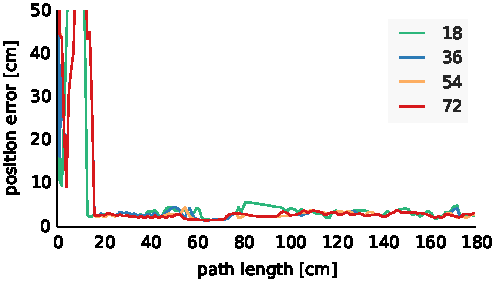
\includegraphics{ml-whole_random_1-xy}\hfill
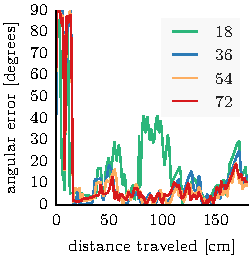
\includegraphics{ml-whole_random_1-theta}

\vspace{.5em}

\begin{center}
Markov Localization, run \texttt{normal 2}
\end{center}
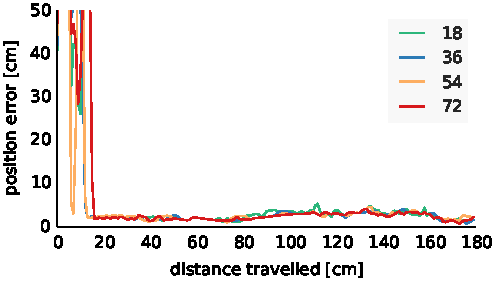
\includegraphics{ml-whole_random_2-xy}\hfill
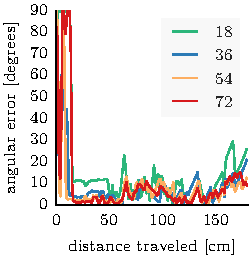
\includegraphics{ml-whole_random_2-theta}

\vspace{.5em}

\begin{center}
Monte Carlo Localization, run \texttt{normal 1}
\end{center}
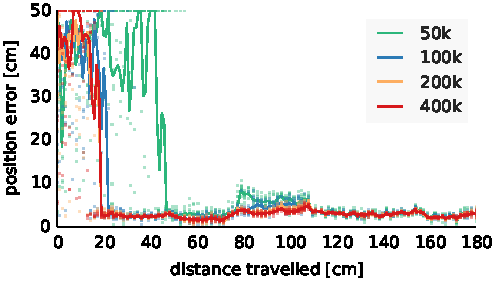
\includegraphics{mcl-whole_random_1-xy}\hfill
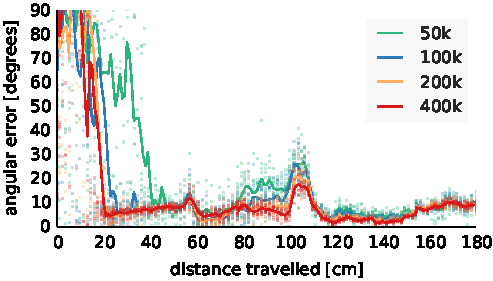
\includegraphics{mcl-whole_random_1-theta}

\vspace{.5em}

\begin{center}
Monte Carlo Localization, run \texttt{normal 2}
\end{center}
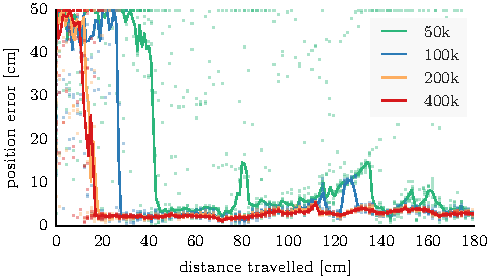
\includegraphics{mcl-whole_random_2-xy}\hfill
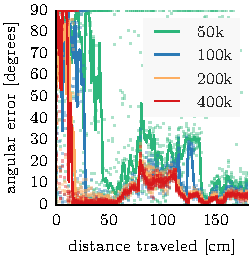
\includegraphics{mcl-whole_random_2-theta}

\caption{The error in position and orientation between the estimation by the localization algorithm and the ground truth, using Markov and Monte Carlo Localization, on two runs.
For Markov Localization, the legend indicates the number of discretization steps for angles; for Monte Carlo Localization, it indicates the number of particles.
For Monte Carlo Localization, the solid lines show the average over 10 trials, while the light dots show the individual trials.
The error is clamped at 50\,cm for position and 90° for orientation.}
\label{fig:whole-runs-random12}
\end{figure*}

\Fig{whole-runs-random12} shows the error in position and orientation for runs \texttt{normal 1} and \texttt{normal 2}.
In these plots, \emph{distance travelled} represents the cumulative distance travelled by the center point between the two ground sensors of the robot.

For Markov Localization approach, all discretization resolutions allow the robot to localize with a precision of 3\,cm and 5°.
In run \texttt{normal 1}, the resolution of 18 is not enough to keep tracking the orientation at distance travelleds 50\,cm and 80\,cm.
These both correspond to the robot rotating on spot.
We see that a discretization of 36 (10° resolution) is sufficient to provide accurate tracking, and that a finer resolution only provides minor improvements in angular precision, and no improvement in position precision.
In run \emph{random\_3}, we see that a resolution of 54 is allows for a better angular precision than 36, but 72 does not improves over 54.
All resolutions provide equal position precision.

For Monte Carlo Localization approach, we see that on run \texttt{normal 1}, the robot localizes already with 50k particles, but twice later than with 100k particles.
Increasing the number of particles over this value only provides minor decrease in localization time and precision.
While 50k particles allow to localize on this run in average, there are some trials (restart of the run) in which the robot looses orientation, when it turns on spot.
On run \texttt{normal 2}, 50k particles is not enough for localizing the robot.
Increasing this number to 100k leads to a good localization, exception during distance travelleds 80--100; indeed this corresponds to a long moment during which the robot rotates on spot, leading to less information acquisition, and therefore degradated precision.

In overall, both approaches have similar localization accuracy.
When angular precision is critical, the Monte Carlo approach might achieve better performance as the Markov approach is limited in precision by its discretization.

%TODO: explain why this does not appear in ML

\subsection{Distance to converge}

\begin{figure*}

\begin{center}
Markov Localization, 10 extracts from \texttt{normal 1} and \texttt{normal 2}
\end{center}
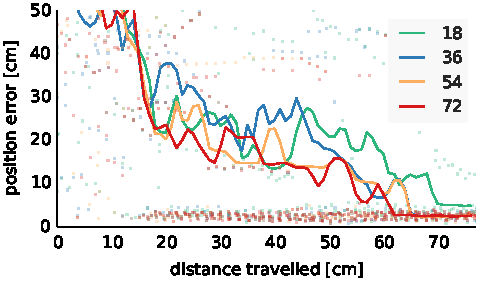
\includegraphics{ml-small_runs_random_12-xy}\hfill
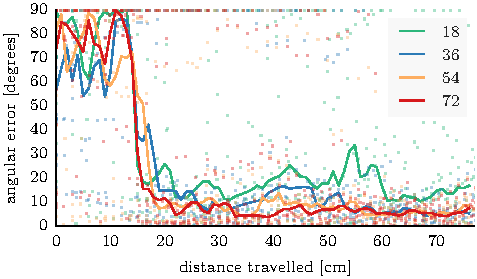
\includegraphics{ml-small_runs_random_12-theta}

\vspace{.5em}

\begin{center}
Monte Carlo Localization, 10 extracts from \texttt{normal 1} and \texttt{normal 2}
\end{center}
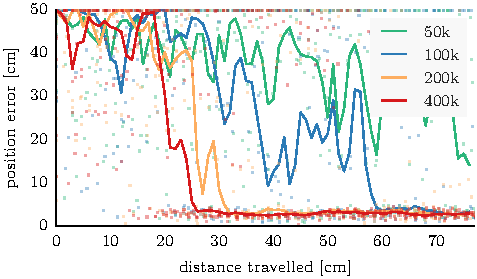
\includegraphics{mcl-small_runs_random_12-xy}\hfill
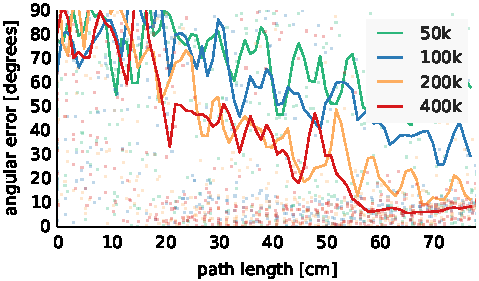
\includegraphics{mcl-small_runs_random_12-theta}

\caption{
The error in position and orientation between the estimation by the localization algorithm and the ground truth, using Markov and Monte Carlo Localization, on 10 extracts from two runs.
For Markov Localization, the legend indicates the number of discretization steps for angles; for Monte Carlo Localization, it indicates the number of particles.
The solid lines show the median over 10 trials, while the light dots show the individual trials.
The error is clamped at 50\,cm for position and 90° for orientation.}
\label{fig:small-runs}
\end{figure*}

\Fig{small-runs} shows the error in position and orientation for 5 different locations in the two normal runs.
We see that, with Markov Localization approach, the correct pose is found after about 20\,cm.
This corresponds well to the ideal theoretical distance of 18\,cm computed in \sect{theoreticalconv}.
However, there are outliers.
This happens when the robot is turning on spot, in that case, there are not enough information to localize the robot.
The convergence is slower with Monte Carlo Localization approach, excepted with 400k particles, in case it is roughly similar.
Decreasing the number of particles quickly increases the distance to converge, reaching 60\,cm for 100k particles.
Using only 50k particles, some extract do not converge even after 80\,cm.

\subsection{Robot kidnapping}

\begin{figure*}

\begin{center}
Markov Localization, run \texttt{kidnapping}
\end{center}
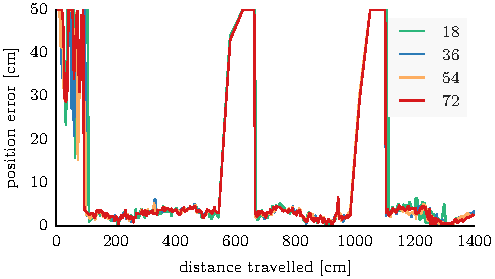
\includegraphics{ml-whole_random_long-xy}\hfill
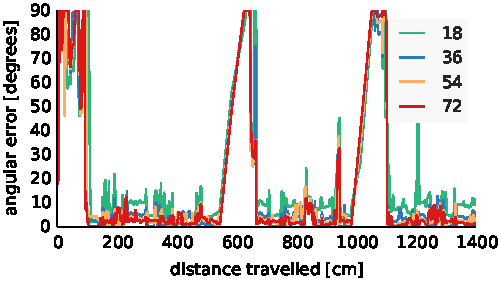
\includegraphics{ml-whole_random_long-theta}

\vspace{.5em}

\begin{center}
Monte Carlo Localization, run \texttt{kidnapping}
\end{center}
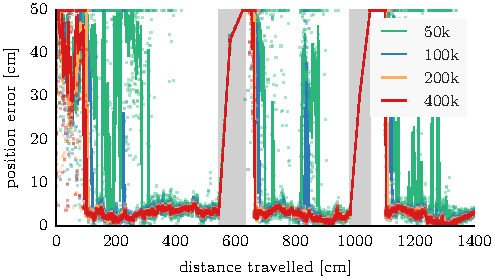
\includegraphics{mcl-whole_random_long-xy}\hfill
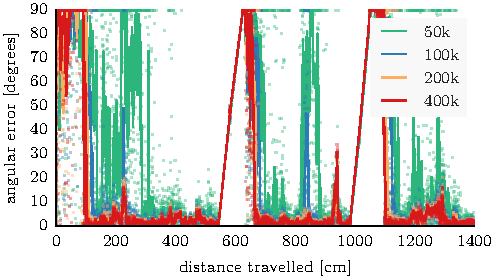
\includegraphics{mcl-whole_random_long-theta}

\caption{The error in position and orientation between the estimation by the localization algorithm and the ground truth, using Markov and Monte Carlo Localization, on the run with kidnapping.
For Markov Localization, the legend indicates the number of discretization steps for angles; for Monte Carlo Localization, it indicates the number of particles.
For Monte Carlo Localization, the solid lines show the median over 10 trials, while the light dots show the individual trials.
The error is clamped at 50\,cm for position and 90° for orientation.}
\label{fig:whole-runs-random-long}
\end{figure*}

\Fig{whole-runs-random-long} shows the error in position and orientation for the run with kidnapping.
In this run, the robot is kidnapped twice, after having travelled 550\,cm and 1000\,cm.
It takes the robot approximately 50\,cm to relocalize, and does so successfully with both Markov and Monte Carlo Localization approaches.
% FIXME: check on the video for numbers, edit plots
With Markov Localization approach, discretization resolutions of 36, 54 and 72 are approximately equivalent in performance, while 18 performs clearly worst, but only for angular resolution.
With Monte Carlo Localization approach, the robot localizes most of the time with 100k particle or more, and always with 200k particles or more.
With 50k particles, the robot eventually localizes, but this might take more than 2 meters of travelled distance.
%TODO: reanalyse MCL once we have 10 runs

\subsection{Computational cost}

\begin{figure}
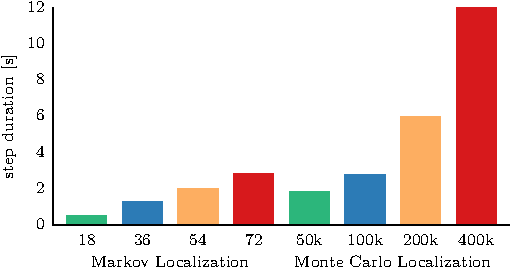
\includegraphics{cpu_load}
\caption{The computational cost for one step for the different implementations.
For Markov Localization, the legend indicates the number of discretization steps for angles; for Monte Carlo Localization, the number of particles.}
\label{fig:cpuload}
\end{figure}

\Fig{cpuload} shows the duration of one step for the different algorithms and parameters, averaged over the two normal runs.
These data were measured on a Lenovo laptop with an Intel XXX processor running at YYY GHz.
We see that with the Markov approach, the duration scales linearly with the number of discretization angles.
With the Monte Carlo approach, the scaling is linear but amortized (50k particles is not twice faster as 100k).
This is due to the selection of pose estimate, which uses a \textsc{ransac} approach and is therefore independant of the number of particles.
For similar localization accuracy, the Monte Carlo approach is slower than the Markov approach, and therefore we suggest to use the former with a discretization angle of 36 in practical applications.
However, the Monte Carlo approach might be prefered if a high angular precision is required.

At a computation duration of 1.5\,s per step, the Monte Carlo Localization approach with a discretization angle of 36 is far from real time.
However, this duration corresponding to a map size of 150\,cm.
If the map would be smaller, for instance 50\,cm, the algorithm would be 9 times faster.
Therefore, at 150\,ms per step, it would be suitable for real-time operations.
Moreover, the code could be further optimized by using multimedia instructions such as \textsc{sse}, implementing it in the \textsc{gpu}, or parallelizing it.
Conditional probability tables are well suited for such optimisations.

%\subsection{Real-time with Thymio}

\section{Discussion}

200k particles is too much

GPU

What works, what does not, why?

Why sampling-based approach is not so easy, but propose how it could be done.

\section{Conclusion}

This paper provides several contributions to the state of the art of localization of robots with low-bandwidth sensors:
\begin{itemize}
\item an empirical evaluation of Markov- and Monte Carlo-based implementations;
\item a method to estimate the localization performance in function of the sensors;
\item a process to let end-users create and provide their own environments, such as drawings made by children.
\end{itemize}
Together, these allow absolute positioning of educational mobile robots in the 100 EUR price range.
This opens many educational opportunities, such as the study of geometry, puzzles based on the physical space, and staging the creation of stories in the context of language education.
These new possibilities are key elements for robots to answer the need for embodied computational thinking education.

\bibliographystyle{IEEEtran}
\bibliography{thymio-localisation-icra}

\end{document}



